\section{Racine RPL}\label{sec:work-rpl-root}
\renewcommand{\rightmark}{Racine RPL}

    Dans la topologie choisie à la section \ref{sec:archi-topologie}, une racine RPL est la plateforme de développement Zolertia RE-Mote Rev.B à laquelle la carte d'interface du RN2483 a été raccordée par des câbles de prototypage. La figure~\ref{fig:work-montage} illustre le raccordement entre le RN2483 et le Zolertia.
    
    \begin{figure}[H]
        \centering
        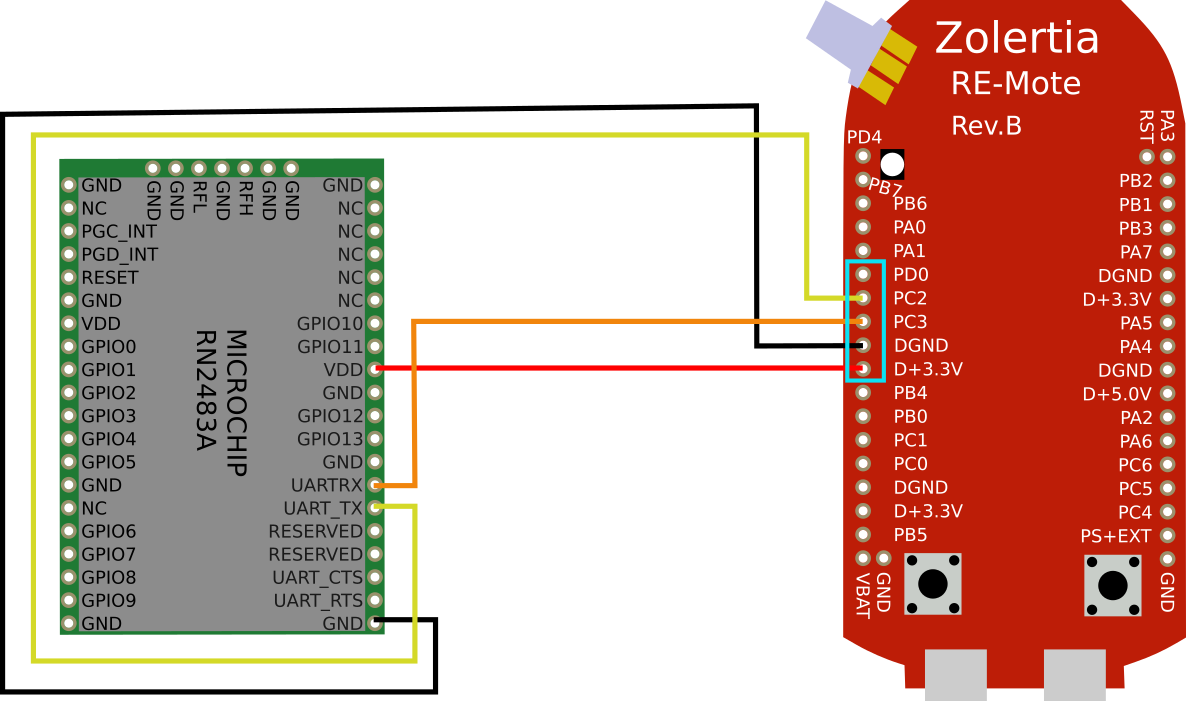
\includegraphics[scale=0.35]{res/pictures/montage.png}
        \caption{Schéma du raccordement du RN2483 au Re-Mote}
        \label{fig:work-montage}
    \end{figure}

    Comme l'indique la table~\ref{table:work-pin-description} de description des pins, les pins PC2 et PC3 utilisés pour la connexion ne sont pas ceux défini pour l'usage d'une connexion UART. Ces pins sont choisis pour la connexion UART car ils sont accessibles à l'exterieur du boitier de la plateforme par un connecteur.
    
    Pour que la connexion UART avec le RN2483 soit possible via les pins choisis, des modifications 
    dans Contiki du fichier de configuration de la plateforme sont nécéssaires.
    Ainsi, les valeurs des macros suivantes ont été modifiées dans le fichier \texttt{arch/cpu/cc2538/cc2538-conf.h}:
    \begin{itemize}
        \item \texttt{UART1\_CONF\_BAUD\_RATE} est définie à $57600$ qui est le baudrate par défaut du RN2483
        \item \texttt{UART1\_RX\_PIN} est définie à $2$
        \item \texttt{UART1\_TX\_PIN} est définie à $3$
    \end{itemize}

    Comme pour l'implémentation de la racine LoRa, celle de la racine RPL est réalisée en 3 couches.
    
    \begin{table}[H]
        \centering
        \makebox[\textwidth]{%
        \begin{tabular}{|l|l|l|l|}
        \hline
        \rowcolor[HTML]{C0C0C0} 
        Pin & Default name       & MC  & Description                                                                            \\ \hline
        4   & UART0.RX           & PA0 & Connected to the CP2104 USB-to-serial converter                                        \\ \hline
        5   & UART0.TX           & PA1 & Connected to the CP2104 USB-to-serial converter                                        \\ \hline
        6   & GPD0/I2C.Interrupt & PD0 & Generic pin, may be used as auxiliary pin for I2C/SPI                                  \\ \hline
        7   & I2C.SDA            & PC2 & \multicolumn{1}{p{10cm}|}{GPIO 20 mA output capability, pull-up. Shared with the RTCC and on-board low-power PIC} \\ \hline
        8   & I2C.SCL            & PC3 &  \multicolumn{1}{p{10cm}|}{GPIO 20 mA output capability, pull-up. Shared with the RTCC and on-board low-power PIC} \\ \hline
        9   & DGND               & N/A & Digital Ground                                                                         \\ \hline
        10  & D+3.3              & N/A & 3.3VDC output pin                                                                      \\ \hline
        11  & CC1200.GPIO0       & PB4 &  \multicolumn{1}{p{10cm}|}{CC1200 GPIO0 pin. If RF switch disables sub-GHz is available for other purposes}        \\ \hline
        12  & CC1200.GPIO2       & PB0 &  \multicolumn{1}{p{10cm}|}{CC1200 GPIO2 pin. If RF switch disables sub-GHz is available for other purposes}        \\ \hline
        13  & UART1.RX           & PC1 &  \multicolumn{1}{p{10cm}|}{GPIO 20 mA output capability, no pull-up or pull-down.}                                 \\ \hline
        14  & UART1.TX           & PC0 &  \multicolumn{1}{p{10cm}|}{GPIO 20 mA output capability, no pull-up or pull-down.  }                               \\ \hline
        \end{tabular}%
        }
        \caption{Extrait de la table de descrition des pins~\cite{zolertia-remote:datasheet}.}
        \label{table:work-pin-description}
        \end{table}
\newpage
\subsection*{Couche physique}
    Comme pour la racine LoRa, la couche physique définit les trame et les adresses LoRaMAC et sert de driver pour le RN2483. La réception et l'envoi de trames UART est réalisée par deux processus.

    Le processus de récéption permet d'éviter que le reste du code soit interrompu par une trame UART entrante. Le code suivant illustre la déclaration de processus dans contiki.  

    \begin{minted}[linenos]{c}
PROCESS_THREAD(ph_rx, ev, data){
    PROCESS_BEGIN();
    /* UART configuration */
    uart_init(UART);
    uart_set_input(UART, &uart_rx);
    PROCESS_END();
}
    \end{minted}
    Tout ce qui se trouve entre les instructions des lignes 2 et 6 dépend du processus. Ainsi, la fonction, \texttt{uart\_rx} qui traite les trames UART entrantes dépend bien de ce processus.
    Le rôle de cette fonction est d'accumuler tous les caractères d'une trame UART pour ensuite appeler une fonctione qui traîte cette trame. Elle supprime également les caractères ayant comme valeur entier 254, 248, 192 et 240. Ces caractèrent apparaissent lors de certaines réponses UART et perturbe la reconstruction de la trame UART. La cause de l'apparition de ces caractères n'est pas identifiée.

    Une fois la trame UART assemblée, une fonction suivante vérifie si la réponse UART est la réponse attendue à la précédente trame envoyée. Si c'est le cas, elle envoie un évènement qu'attend le processus d'envoi pour envoyer la prochaine trame UART. Si la trame UART reçue contient la commande \textit{"radio\_rx"}, la fonction construit une trame LoRaMAC et l'envoie à la couche supérieure.

    Le processus d'envoi apour rôle d'envoyer toutes les trames UART présentes dans le buffer 
    d'envoi. Il peut être bloqué si le buffer d'envoi est vide ou s'il attend une réponse à la 
    dernière trame envoyée. Si le buffer est d'envoi est vide, le processus sera débloqué par la 
    réception de l'évènement \texttt{new\_tx\_frame\_event}, et s'il attend une réponse, il sera 
    débloqué par la réception de l'évènement \texttt{can\_send\_event}.

    Dans Contiki, les évènements sont créés et envoyé de la manière suivante:
    \begin{minted}[linenos]{c}
        process_event_t new_tx_frame_event = process_alloc_event();
        process_post(&ph_tx, new_tx_frame_event, NULL);
    \end{minted}
    
    Le type type \texttt{process\_event\_t} est en réalité un \texttt{unsigned char} qui est incrémenté à chaque appel de \texttt{process\_alloc\_event()}.

    Les fonctions publiques de la couche physique sont les suivantes:
    \begin{itemize}
        \item \texttt{void phy\_init()}\\
            Initialise la couche physique. C'est à dire, alloue les évènements, démarre les processus et envoie les trames UART permettant de mettre en pause LoRaWAN et de définir la fréquence.
        \item \texttt{void phy\_register\_listener(int (* listener)(lora\_frame\_t frame))}\\
            Enregistre la fonction callback qui sera appelée lorsqu'une trame LoRaMAC est reçue.
        \item \texttt{int phy\_tx(lora\_frame\_t frame)}\\
            Envoie une trame LoRaMAC.
        \item \texttt{int phy\_timeout(int timeout)}\\
            Définis le temps d'expiration du watchdog timer.
        \item \texttt{int phy\_sleep(int duration)}\\
            Met le RN2483 en mode sommeil.
        \item \texttt{int phy\_rx()}\\
            Met le RN2483 en mode sommeil.
    \end{itemize}

    Toues ces fonctions créent une trame UART qu'elle ajoute au buffer d'envoi.

\subsection*{Couche MAC}
    %todo
\subsection*{Couche IP}
    %todo
% Please add the following required packages to your document preamble:
% \usepackage{graphicx}
% \usepackage[table,xcdraw]{xcolor}
% If you use beamer only pass "xcolor=table" option, i.e. \documentclass[xcolor=table]{beamer}
